% 34-21(34쪽) — $y=4^{x}$, $y=a^{x}$ 의 그래프와 직선 $y=k$, 네 점 $\pt{A}$·$\pt{B}$·$\pt{C}$·$\pt{D}$(원문 「오른쪽 그림」). 스캔 화질이 낮아 TikZ 로 다시 그림.
% 두 삼각형(원문의 색칠)은 원문처럼 삼각형 $\pt{ACB}$ 를 주황, 삼각형 $\pt{ADC}$ 를 하늘색으로 칠한다.
% 라벨은 원문 것만: 두 그래프 이름, 직선 이름 $y=k$, 네 점 이름, $\pt{O}$. $a$ 의 값(답)이 읽히지 않게 눈금·좌표값은 적지 않는다.
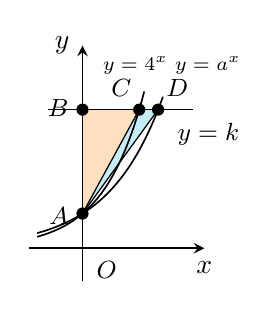
\begin{tikzpicture}[line width=0.6pt, x=0.72cm, y=0.44cm, >=stealth]
  \fill[orange!25] (0,1) -- (0,4) -- (1,4) -- cycle;
  \fill[cyan!22] (0,1) -- (1,4) -- (1.3333,4) -- cycle;
  \draw[->, line width=0.7pt] (-0.95,0) -- (2.15,0) node[below=1pt] {$x$};
  \draw[->, line width=0.7pt] (0,-0.95) -- (0,5.85) node[left=1pt] {$y$};
  \draw[line width=0.5pt] (-0.60,4) -- (1.95,4);
  \draw[line width=0.45pt] (0,1) -- (1,4);
  \draw[line width=0.45pt] (0,1) -- (1.3333,4);
  \draw[domain=-0.80:1.09, samples=90, smooth] plot (\x, {pow(4,\x)});
  \draw[domain=-0.80:1.42, samples=90, smooth] plot (\x, {exp(1.0397*\x)});
  \fill (0,1) circle (2.2pt);
  \fill (0,4) circle (2.2pt);
  \fill (1,4) circle (2.2pt);
  \fill (1.3333,4) circle (2.2pt);
  \node[anchor=east, font=\small] at (-0.07,0.92) {$\pt{A}$};
  \node[anchor=east, font=\small] at (-0.07,4.05) {$\pt{B}$};
  \node[anchor=south east, font=\small] at (1.04,4.10) {$\pt{C}$};
  \node[anchor=south west, font=\small] at (1.30,4.10) {$\pt{D}$};
  \node[anchor=north west, font=\small] at (1.50,3.90) {$y=k$};
  \node[anchor=north west, font=\small] at (0.07,-0.08) {$\pt{O}$};
  \node[anchor=south west, font=\scriptsize] at (0.18,4.72) {$y=4^{x}$};
  \node[anchor=south west, font=\scriptsize] at (1.45,4.72) {$y=a^{x}$};
\end{tikzpicture}
